\documentclass[./../main_file.tex]{subfiles}

\begin{document}

Nhóm đã vận dụng và kết hợp hai phương pháp thiết kế Inside-out và Outside-in để xác định các tiến trình và phân bổ các lớp thiết kế, hệ thống con vào các tiến trình và luồng phù hợp. Kết quả được phân tích ở nội dung bên dưới.

\subsection{Đăng nhập hệ thống}

\subsubsection{Mô hình tiến trình}

\begin{figure}[H]
	\centering
	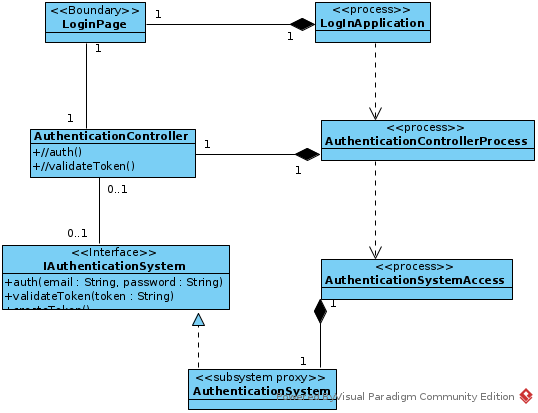
\includegraphics[width=\linewidth]{./images/pv_login.png}
\end{figure}

\subsubsection{Mô tả các phần tử tiến trình}
\begin{itemize}
	\item Tiến trình LoginApplication: Điều khiển giao diện, biểu mẫu cho người dùng (sinh viên, giảng viên và quản trị viên) đăng nhập vào hệ thống để có thể sử dụng các dịch vụ. Tiến trình này có thể hiện của lớp LogInPage có nhiệm vụ giúp người dùng đăng nhập vào hệ thống.
	      Một thể hiện của tiến trình này ứng với một khách đăng nhập vào hệ thống
	\item Tiến trình AuthenticationControllerProcess: Quản lý quá trình thực hiện xác thực tài khoản của người dùng bao gồm sinh viên, giảng viên và quản trị viên hệ thống.
	      Một thể hiện của tiến trình này tương ứng với mỗi lần khách đăng nhập hệ thống.
	\item Tiến trình AuthenticationSystemAccess: Quản lý tất cả truy cập đến hệ thống con AuthenticationSystem.
	      Chỉ có một thể hiện của tiến trình AuthenticationSystemAccess.
\end{itemize}

\subsection{Quản lý thông tin cá nhân}

\subsubsection{Mô hình tiến trình}

\begin{figure}[H]
	\centering
	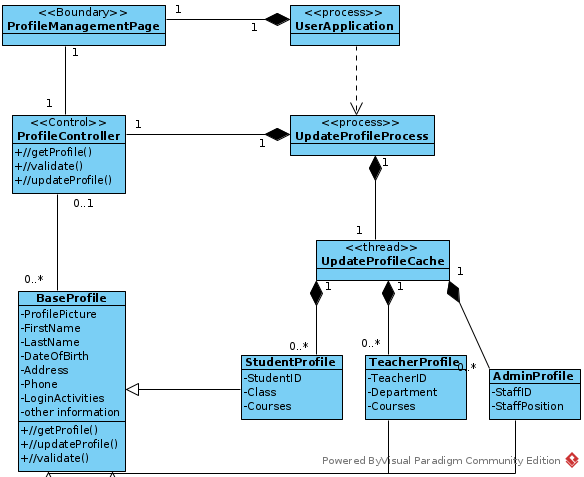
\includegraphics[width=\linewidth]{./images/pv_ProfileManagement.png}
\end{figure}

\subsubsection{Mô tả các phần tử tiến trình}
\begin{itemize}
	\item Tiến trình UserApplication: Điều khiển các giao diện, biểu mẫu dành cho người dùng có thể thao tác và sử dụng các dịch vụ của hệ thống. Trong tiến trình này có  thể hiện của lớp ProfileManagementPage có nhiệm vụ giúp người dùng có thể xem và cập nhật thông tin cá nhân của mình trên hệ thống.
	      Một thể hiện của tiến trình này tương ứng với mỗi người dùng truy cập hệ thống.
	\item Tiến trình UpdateProfileProcess: Quản lý quá trình thực hiện xử lý cập nhật thông tin cá nhân của người dùng trên hệ thống.
	      Một thể hiện của tiến trình này tương ứng với mỗi lần người dùng thay đổi, cập nhật thông tin cá nhân trên hệ thống.
	\item Luồng UpdateProfileCache: Đóng gói một yêu cầu cập nhật thông tin cá nhân của người dùng trên hệ thống.
\end{itemize}

\subsection{Đăng Blog}

\subsubsection{Mô hình tiến trình}

\begin{figure}[H]
	\centering
	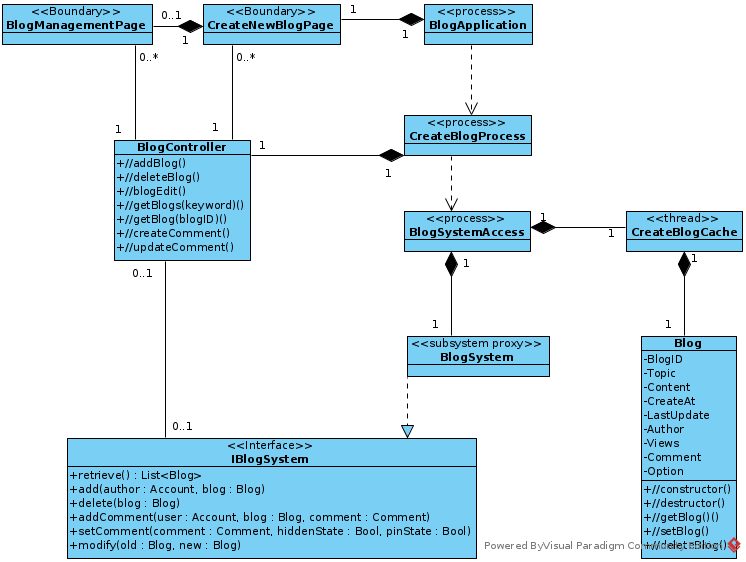
\includegraphics[width=\linewidth]{./images/pv_Blog.png}
\end{figure}

\subsubsection{Mô tả các phần tử tiến trình}
\begin{itemize}
	\item Tiến trình BlogApplication: Điều khiển các giao diện, biểu mẫu dành cho người dùng có thể thao tác và sử dụng các dịch vụ của hệ thống. Trong tiến trình này có thể hiện của lớp CreateNewBlogPage có nhiệm vụ giúp người dùng có thể tạo mới một bài đăng trên hệ thống và lớp BlogManagementPage có nhiệm vụ giúp người dùng quản lý các bài đăng của mình trên hệ thống.
	      Một thể hiện của tiến trình này tương ứng với mỗi người dùng truy cập hệ thống.
	\item Tiến trình CreateBlogProcess: Quản lý quá trình thực hiện xử lý tạo mới một bài đăng của người dùng lên trên hệ thống.
	      Một thể hiện của tiến trình này tương ứng với mỗi lần người dùng tạo mới một bài đăng trên hệ thống.
	\item Tiến trình BlogSystemAccess: Quản lý tất cả các truy cập đến hệ thống con BlogSystem. Vì quy trình cập nhật này có thể mất nhiều thời gian nên điều này cho phép người dùng có thể tiến hành các thao tác khác trên hệ thống trong quá trình chờ phản hồi từ hệ thống con BlogSystem. Tiến trình này cũng đồng bộ hóa quyền truy cập vào hệ thống con BlogSystem từ các tiến trình hệ thống khác.
	      Chỉ có một thể hiện của tiến trình BlogSystemAccess.
	\item Luồng CreateBlogCache: Đóng gói một yêu cầu tạo mới một bài đăng của người dùng trên hệ thống.
\end{itemize}

\subsection{Nhắn tin}

\subsubsection{Mô hình tiến trình}

\begin{figure}[H]
	\centering
	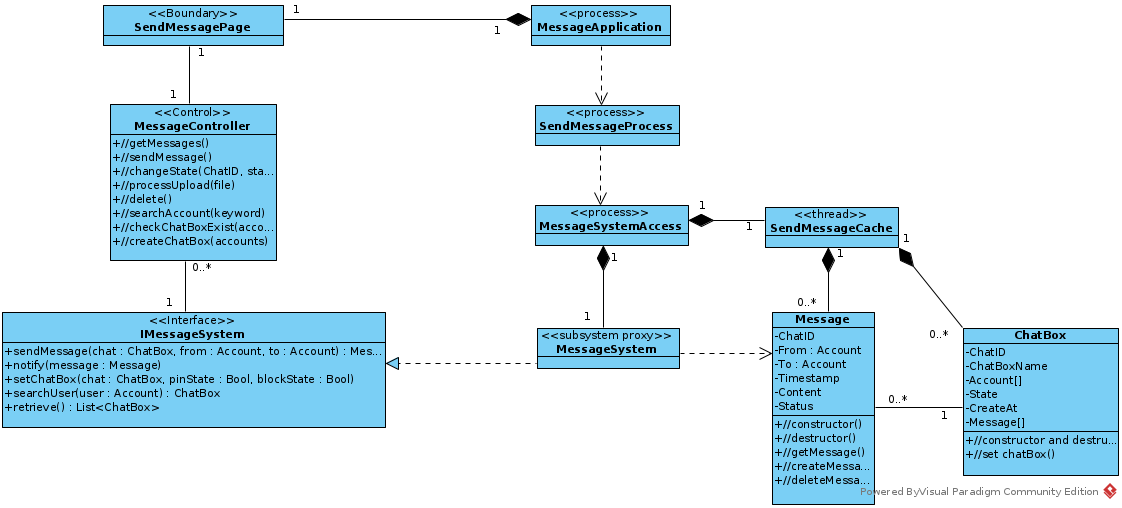
\includegraphics[width=\linewidth]{./images/pv_Message.png}
\end{figure}

\subsubsection{Mô tả các phần tử tiến trình}
\begin{itemize}
	\item Tiến trình MessageApplication: Điều khiển các giao diện, biểu mẫu dành cho người dùng hệ thống để có thể thao tác, sử dụng các dịch vụ của hệ thống. Tiến trình này có một thể hiện của lớp SendMessagePage có nhiệm vụ giúp người dùng tiến hành thao tác nhắn tin với người dùng khác trên hệ thống.
	Một thể hiện của tiến trình này tương ứng với mỗi người dùng sử dụng hệ thống.
	\item Tiến trình SendMessageProcess: Quản lý quá trình thực hiện xử lý nhắn tin với người dùng khác trên hệ thống.
	Một thể hiện của tiến trình này tương ứng với mỗi lần nhắn tin với người dùng khác trên hệ thống.
	\item Tiến trình MessageSystemAccess: Quản lý tất cả các hoạt động truy cập tới hệ thống con MessageSystem. Vì quá trình truy cập này có thể mất nhiều thời gian nên điều này cho phép người dùng có thể tiến hành các thao tác khác trên hệ thống trong quá trình chờ phản hồi từ hệ thống con MessageSystem. Tiến trình này cũng đồng bộ hóa quyền truy cập vào hệ thống con MessageSystem từ các tiến trình hệ thống khác.
	Chỉ có một thể hiện của tiến trình MessageSystemAccess.
	\item Luồng SendMessageCache: Đóng gói một yêu cầu nhắn tin của người dùng trên hệ thống.
\end{itemize}

\subsection{Tham gia lớp học}

\subsubsection{Mô hình tiến trình}

\begin{figure}[H]
	\centering
	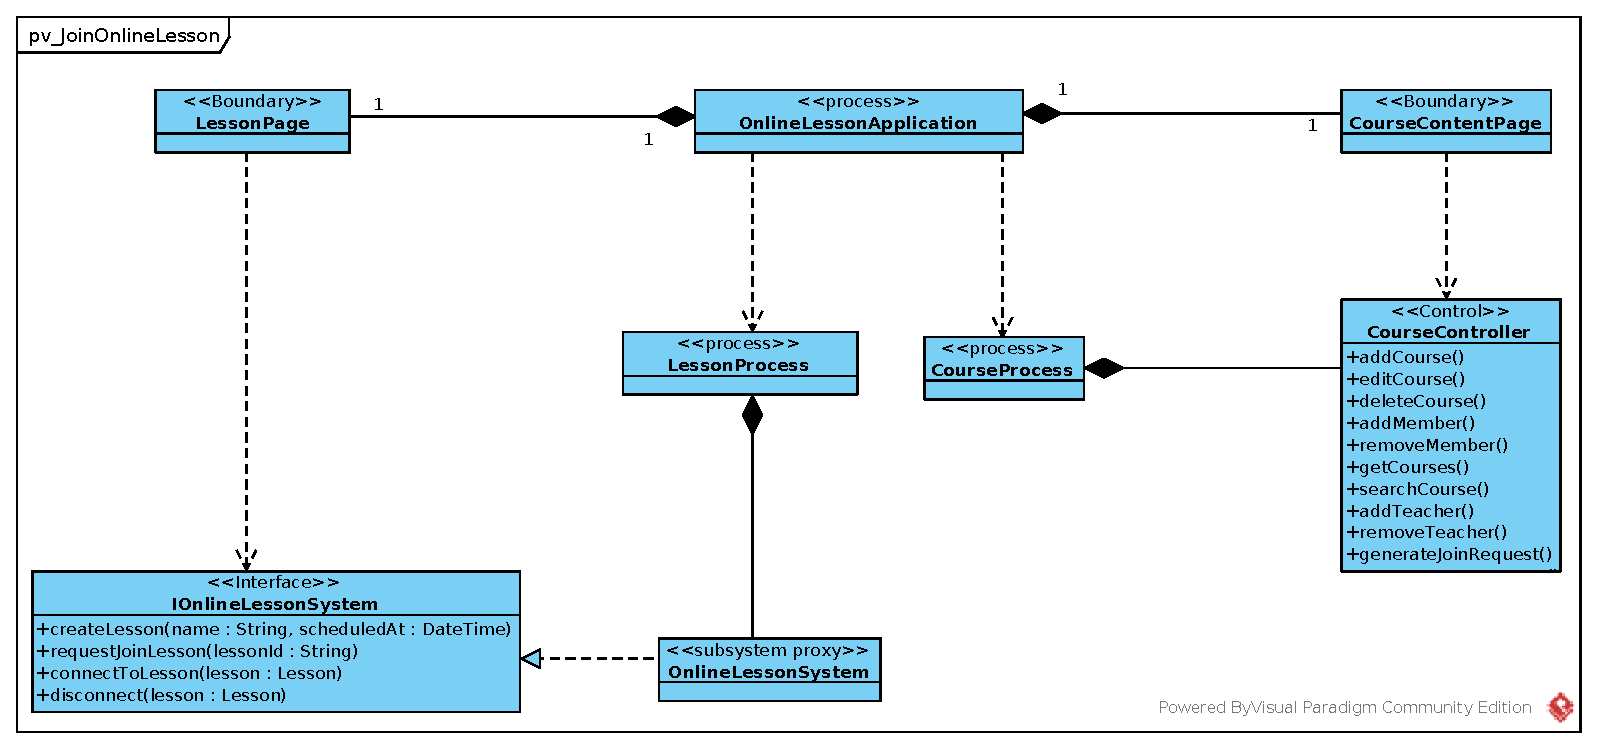
\includegraphics[width=\linewidth]{./images/pv_JoinOnlineLesson.eps}
\end{figure}

\subsubsection{Mô tả các phần tử tiến trình}
\begin{itemize}
	\item Tiến trình OnlineLessonApplication: Điều khiển các giao diện, biểu mẫu dành cho người dùng hệ thống để có thể thao tác, sử dụng các dịch vụ của hệ thống. Tiến trình này có một thể hiện của lớp CourseContentPage có nhiệm vụ giúp người dùng truy cập vào lớp học của trực tuyến thông qua các khóa học và LessonPage cung cấp giao diện người dùng sử dụng các thao tác trên hệ thống.
	Mỗi thể hiện tiến trình này tương ứng với một người dùng.
	\item Tiến trình CourseProcess: quản lý và điều hướng người dùng tới ứng dụng lớp học trực tuyến.
	Mỗi thể hiện tiến trình này tương ứng với một người dùng.
	\item Tiến trình LessonProcess: quản lý và thực hiện các thao tác của người dùng tới  hệ thống con OnlineLessonSystem.
	Mỗi thể hiện tiến trình này tương ứng với một người dùng.
	
\end{itemize}

\subsection{Tìm kiếm và khám phá}

\subsubsection{Mô hình tiến trình}

\begin{figure}[H]
	\centering
	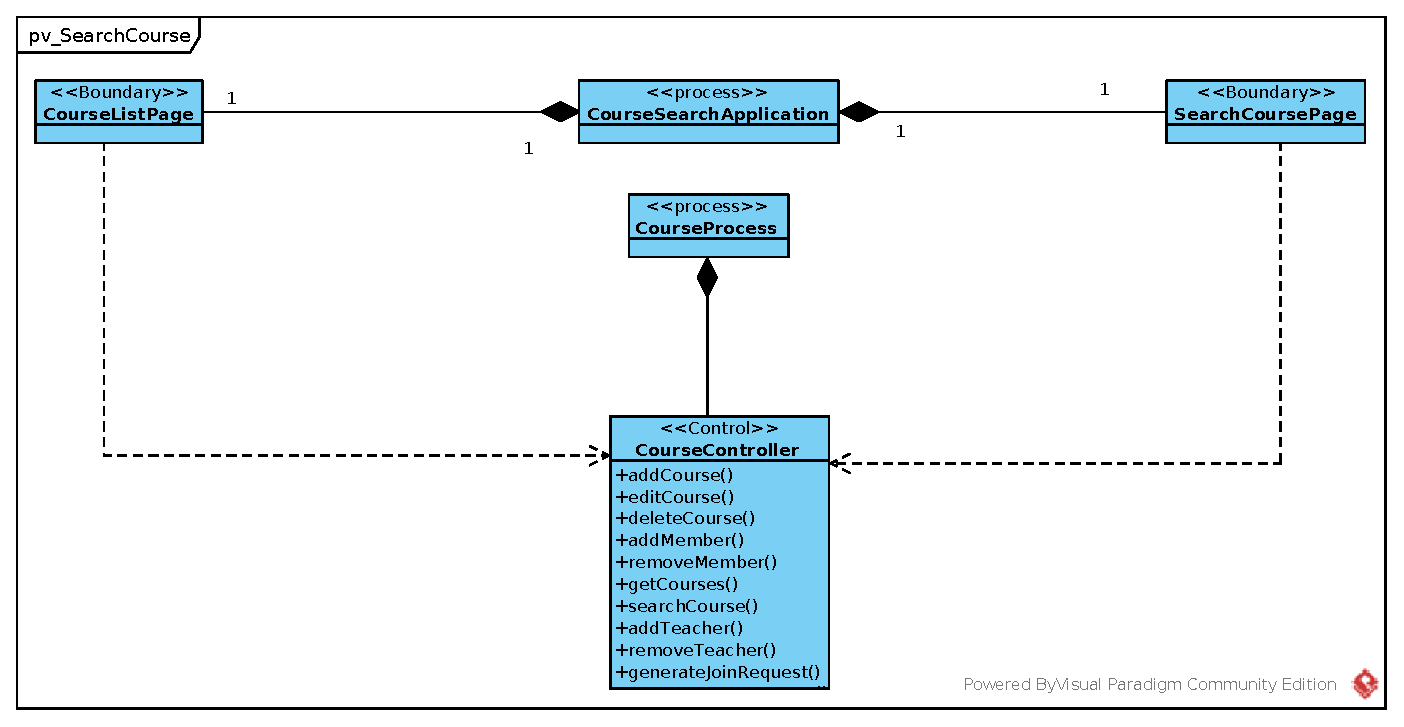
\includegraphics[width=\linewidth]{./images/pv_SearchCourse.eps}
\end{figure}

\subsubsection{Mô tả các phần tử tiến trình}
\begin{itemize}
	\item Tiến trình CourseSearchApplication: Điều khiển các giao diện, biểu mẫu dành cho người dùng hệ thống để có thể thao tác, sử dụng các dịch vụ của hệ thống. Tiến trình này có một thể hiện của lớp SearchCousePage có nhiệm vụ giúp người sử dụng các thao tác tìm kiếm trên ứng dụng và CourseListPage cung cấp giao diện giúp người dùng sử dụng và lấy các thông tin về khóa học trong kết quả tìm kiếm.
	Mỗi thể hiện tiến trình này tương ứng với một người dùng.
	\item Tiến trình CourseProcess: Quản lý quá trình thực hiện tìm kiếm trên hệ thống.
	Mỗi thể hiện tiến trình này tương ứng với một người dùng.
	
\end{itemize}

\subsection{Thảo luận trực tuyến}

\subsubsection{Mô hình tiến trình}

\begin{figure}[H]
	\centering
	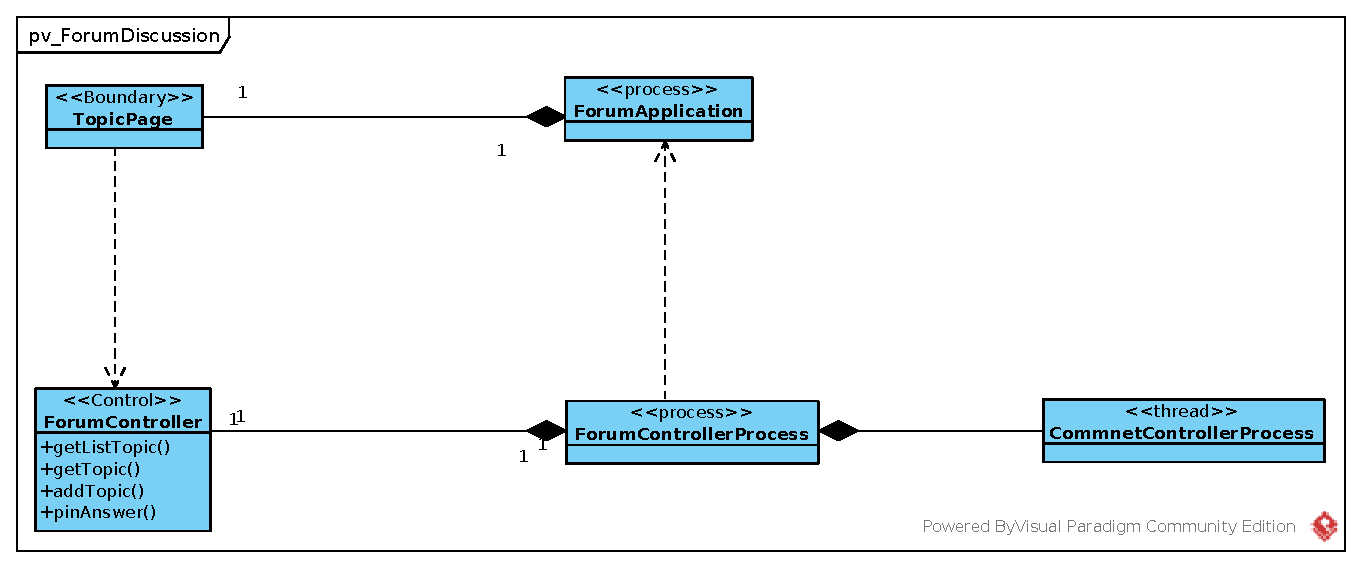
\includegraphics[width=\linewidth]{./images/pv_ForumDiscussion.eps}
\end{figure}

\subsubsection{Mô tả các phần tử tiến trình}
\begin{itemize}
	\item Tiến trình ForumApplication: : Điều khiển các giao diện, biểu mẫu dành cho người dùng hệ thống để có thể thao tác, sử dụng các dịch vụ của hệ thống. Tiến trình này có một thể hiện của lớp TopicPage cung cấp giao diện về chủ đề đang thảo luận.
	Mỗi thể hiện tiến trình này tương ứng với một người dùng.
	\item Tiến trình ForumControllerProcess: Quá trình thực hiện các thao tác trong chủ đề với hệ thống .
	Mỗi thể hiện tiến trình này tương ứng với một người dùng.
	\item Luồng CommentControllerThread thực hiện đóng gói, gửi và cập nhập các bình luận trong chủ đề một cách liên tục.
	
\end{itemize}

\subsection{Thực hiện kiểm tra trực tuyến}

\subsubsection{Mô hình tiến trình}

\begin{figure}[H]
	\centering
	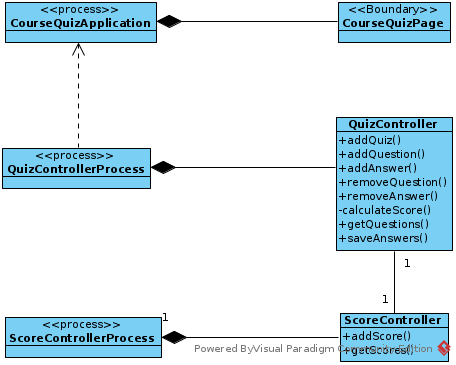
\includegraphics[width=\linewidth]{./images/pv_take_test.png}
\end{figure}

\subsubsection{Mô tả các phần tử tiến trình}
\begin{itemize}
	\item Tiến trình CourseQuizApplication: Quản lý giao diện bài kiểm tra trong một khóa học.
	\item Tiến trình QuizControllerProcess: Quản lý danh sách bài kiểm tra, danh sách câu hỏi trong bài kiểm tra đó và thực hiện tính toán điểm số.
	\item Tiến trình ScoreControllerProcess: Quản lý việc lưu trữ điểm thi.
	
\end{itemize}

\subsection{Nộp bài tập}

\subsubsection{Mô hình tiến trình}

\begin{figure}[H]
	\centering
	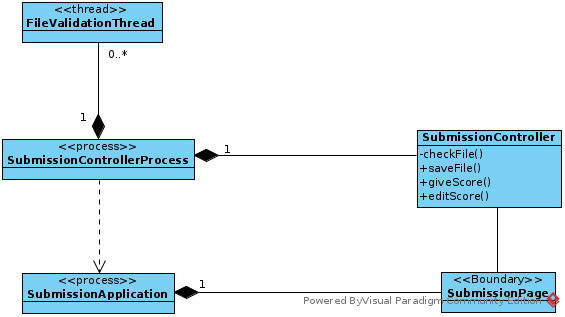
\includegraphics[width=\linewidth]{./images/pv_submit_assignment.png}
\end{figure}

\subsubsection{Mô tả các phần tử tiến trình}

\begin{itemize}
	\item Tiến trình SubmissionControllerProcess: Quản lý xử lý và lưu trữ file bài nộp do học sinh upload lên hệ thống.
	\item Tiến trình SubmissionApplication: Quản lý giao diện nộp bài tập.
	\item Luồng FileValidationThread: Kiểm tra file được upload có thỏa mãn yêu cầu của hệ thống hay không (kiểu file, kích thước, số lượng, …).
\end{itemize}

\subsection{Khám phá khóa học}

\subsubsection{Mô hình tiến trình}

\begin{figure}[H]
	\centering
	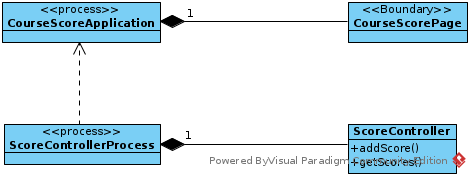
\includegraphics[width=\linewidth]{./images/pv_check_course_progress.png}
\end{figure}

\subsubsection{Mô tả các phần tử tiến trình}

\begin{itemize}
	\item Tiến trình ScoreControllerProcess: Quản lý việc lưu trữ và đọc điểm thi của người dùng.
	\item Tiến trình CourseScoreApplication: Quản lý giao diện xem điểm thi cho người dùng hệ thống.
\end{itemize}

\subsection{Đánh giá khóa học}

\subsubsection{Mô hình tiến trình}

\begin{figure}[H]
	\centering
	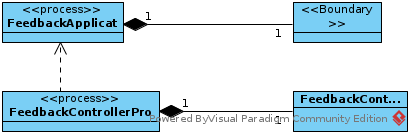
\includegraphics[width=\linewidth]{./images/pv_feedback_course.png}
\end{figure}

\subsubsection{Mô tả các phần tử tiến trình}

\begin{itemize}
	\item Tiến trình FeedbackApplication: Quản lý giao diện gửi feedback về khóa học.
	\item Tiến trình FeedbackControllerProcess: Quản lý xử lý và gửi feedback khóa học.
\end{itemize}

\subsection{Quản lý hoạt động sinh viên}

\subsubsection{Mô hình tiến trình}

\begin{figure}[H]
	\centering
	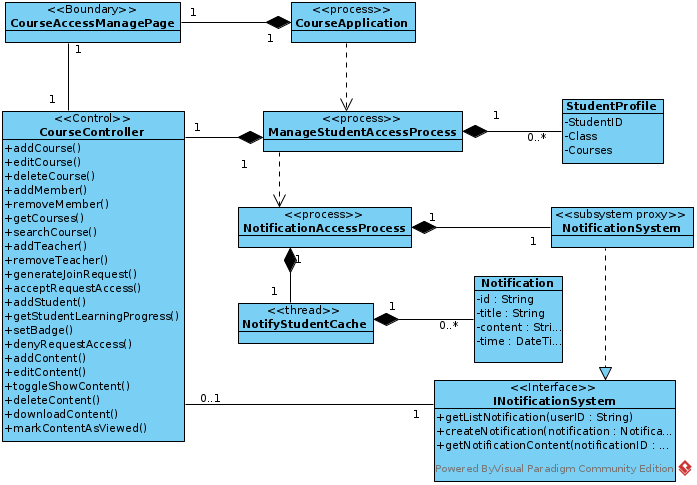
\includegraphics[width=\linewidth]{./images/pv_manage_studentactivity.png}
\end{figure}

\subsubsection{Mô tả các phần tử tiến trình}
\begin{itemize}
	\item Tiến trình CourseApplication: Điều khiển các giao diện, biểu mẫu dành cho người dùng hệ thống để có thể thao tác, sử dụng các dịch vụ của hệ thống. Tiến trình này có một thể hiện của lớp CourseAccessManagePage có nhiệm vụ giúp giảng viên tiến hành thao tác chấp nhận hoặc từ chối yêu cầu truy cập vào khóa học của sinh viên.
	Một thể hiện của tiến trình này tương ứng với mỗi giảng viên sử dụng hệ thống.
	\item Tiến trình ManageStudentAccessProcess: Quản lý quá trình thực hiện xử lý quyền truy cập của sinh viên vào lớp học phần.
	Một thể hiện của tiến trình này tương ứng với mỗi lần giảng viên phản hồi yêu cầu truy cập vào lớp học phần của sinh viên.
	\item Tiến trình NotificationSystemAccess: Quản lý tất cả các hoạt động truy cập tới hệ thống con NotificationSystem. Vì quá trình truy cập này có thể mất nhiều thời gian nên điều này cho phép người dùng có thể tiến hành các thao tác khác trên hệ thống trong quá trình chờ phản hồi từ hệ thống con NotificationSystem. Tiến trình này cũng đồng bộ hóa quyền truy cập vào hệ thống con NotificationSystem từ các tiến trình hệ thống khác.
	Chỉ có một thể hiện của tiến trình NotificationSystemAccess.
	\item Luồng NotifyStudentCache: Đóng gói một yêu cầu thông báo tới sinh viên về quyền truy cập lớp học phần mà giảng viên đã phản hồi.
\end{itemize}

\subsection{Quản lý hoạt động diễn đàn}

\subsubsection{Mô hình tiến trình}

\begin{figure}[H]
	\centering
	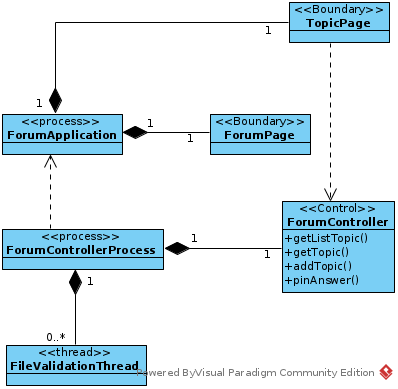
\includegraphics[width=\linewidth]{./images/pv_manage_forum.png}
\end{figure}

\subsubsection{Mô tả các phần tử tiến trình}
\begin{itemize}
	\item Tiến trình ForumApplication: Quản lý giao diện Forum và Topic.
	\item Tiến trình ForumControllerProcess: Quản lý việc tạo Forum, đăng topic trong forum và bình luận topic.
	\item Luồng FileValidationThread: Thực hiện kiểm tra file với các topic có đính kèm file.
\end{itemize}

\subsection{Quản lý nội dung khóa học}

\subsubsection{Mô hình tiến trình}

\begin{figure}[H]
	\centering
	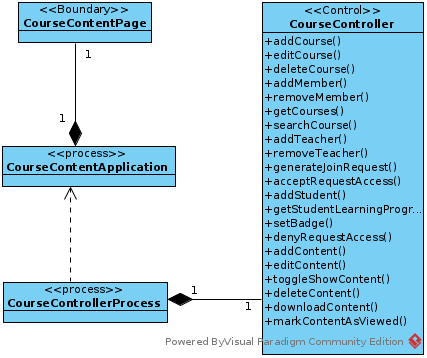
\includegraphics[width=\linewidth]{./images/pv_manage_contentcourse.png}
\end{figure}

\subsubsection{Mô tả các phần tử tiến trình}
\begin{itemize}
	\item Tiến trình CourseContentApplication: Quản lý giao diện nội dung khóa học.
	\item Tiến trình CourseControllerProcess: Quản lý việc tạo mới và chỉnh sửa nội dung khóa học.
\end{itemize}

\subsection{Quản lý danh sách sinh viên}

\subsubsection{Mô hình tiến trình}

\begin{figure}[H]
	\centering
	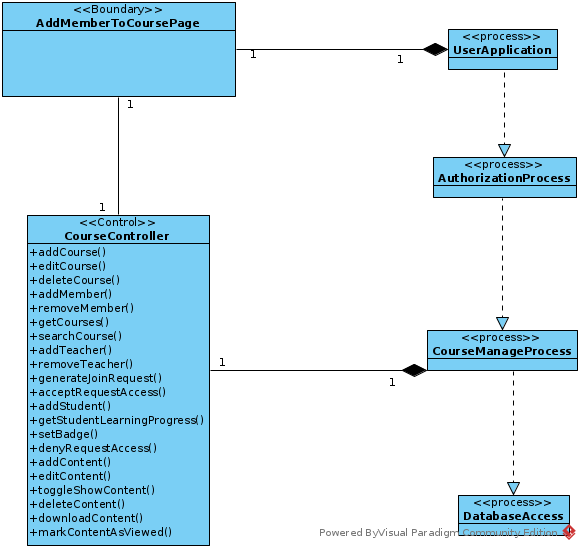
\includegraphics[width=\linewidth]{./images/pv_add_course_member.png}
\end{figure}

\subsubsection{Mô tả các phần tử tiến trình}
\begin{itemize}
	\item Tiến trình UserApplication: Cung cấp giao diện, chức năng liên quan đến người dùng trong hệ thống. Có một thể hiện của tiến trình này tương ứng với mỗi khách đăng nhập hệ thống.
	\item Tiến trình AuthorizationProcess: Quản lý quá trình thực hiện kiểm tra quyền truy cập tài khoản người dùng.
	Có một thể hiện của tiến trình này tương ứng mỗi lần khách truy cập trên hệ thống.
\item Tiến trình CourseManageProcess: Quản lý quá trình xử lý các yêu cầu liên quan tới khóa học.
	Có một thể hiện cho mỗi yêu cầu người dùng lên hệ thống.
	\item Tiến trình DatabaseAccess: Quản lý, xử lý các yêu cầu và thao tác liên quan đến database của hệ thống. Có nhiều thể hiện của tiến trình tương ứng với các database của hệ thống kết nối đến.
\end{itemize}

\subsection{Quản lý dạy học trực tuyến}

\subsubsection{Mô hình tiến trình}

\begin{figure}[H]
	\centering
	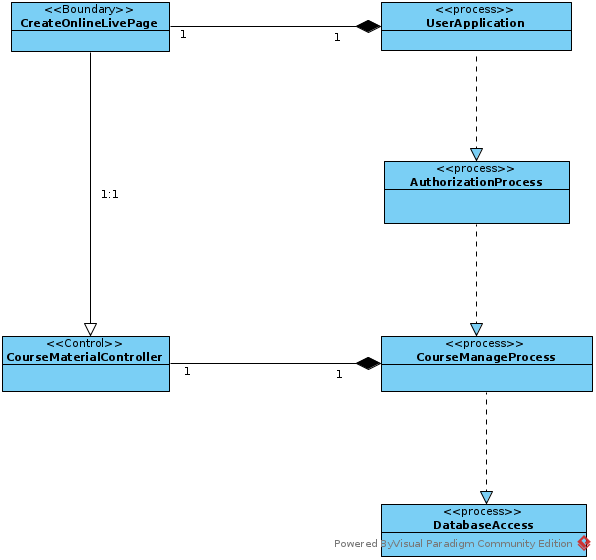
\includegraphics[width=\linewidth]{./images/pv_create_online_live.png}
\end{figure}

\subsubsection{Mô tả các phần tử tiến trình}
\begin{itemize}
	\item Tiến trình UserApplication: Cung cấp giao diện, chức năng liên quan đến người dùng trong hệ thống. Có một thể hiện của tiến trình này tương ứng với mỗi khách đăng nhập hệ thống.
	\item Tiến trình AuthorizationProcess: Quản lý quá trình thực hiện kiểm tra quyền truy cập tài khoản người dùng.
	Có một thể hiện của tiến trình này tương ứng mỗi lần khách truy cập trên hệ thống.
\item Tiến trình CourseManageProcess: Quản lý quá trình xử lý các yêu cầu liên quan tới khóa học (ở đây là tạo một lớp học trực tuyến mới).
	Có một thể hiện cho mỗi yêu cầu người dùng lên hệ thống.
	\item Tiến trình DatabaseAccess: Quản lý, xử lý các yêu cầu và thao tác liên quan đến  database của hệ thống. Có nhiều thể hiện của tiến trình tương ứng với các database của hệ thống kết nối đến.
\end{itemize}

\subsection{Quản lý tài khoản}

\subsubsection{Mô hình tiến trình}

\begin{figure}[H]
	\centering
	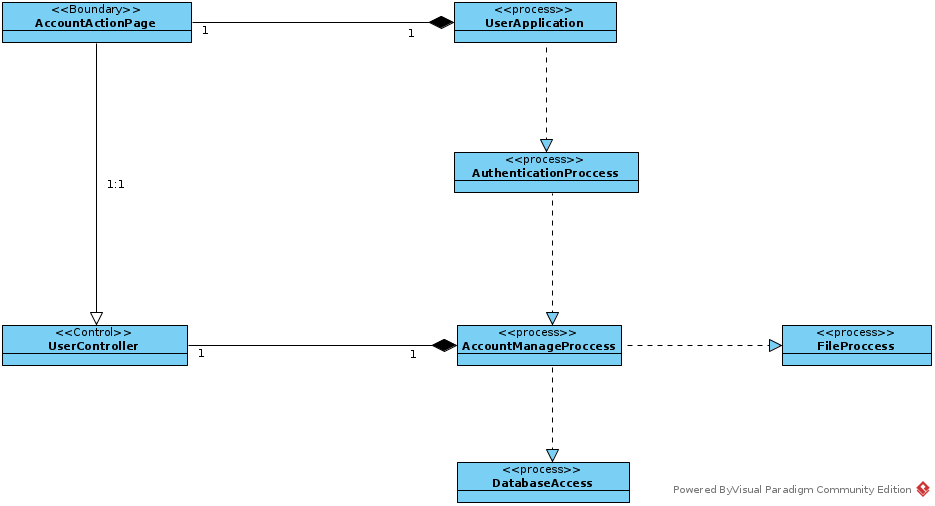
\includegraphics[width=\linewidth]{./images/pv_account_manage.png}
\end{figure}

\subsubsection{Mô tả các phần tử tiến trình}
\begin{itemize}
	\item Tiến trình UserApplication: Cung cấp giao diện, chức năng liên quan đến người dùng trong hệ thống. Có một thể hiện của tiến trình này tương ứng với mỗi khách đăng nhập hệ thống.
	\item Tiến trình AuthenticationProcess: Quản lý quá trình thực hiện xử lý tạo, xác thực tài khoản người dùng.
	Có một thể hiện của tiến trình này tương ứng mỗi lần khách truy cập đăng ký tài khoản/đăng nhập trên hệ thống.
\item Tiến trình AccountManageProcess: Quản lý các thực hiện, xử lý liên quan đến tài khoản người dùng.
	Có một thể hiện của tiến trình này tương ứng mỗi lần khách yêu cầu xử lý tài khoản.
	\item Tiến trình FileProcess: Quản lý, xử lý các tác vụ với tệp.
	Có một tiến trình cho toàn bộ hệ thống.
	\item Tiến trình DatabaseAccess: Quản lý, xử lý các yêu cầu và thao tác liên quan đến database của hệ thống. Có nhiều thể hiện của tiến trình tương ứng với các database của hệ thống kết nối đến.
\end{itemize}

\subsection{Quản lý danh sách khóa học}

\subsubsection{Mô hình tiến trình}

\begin{figure}[H]
	\centering
	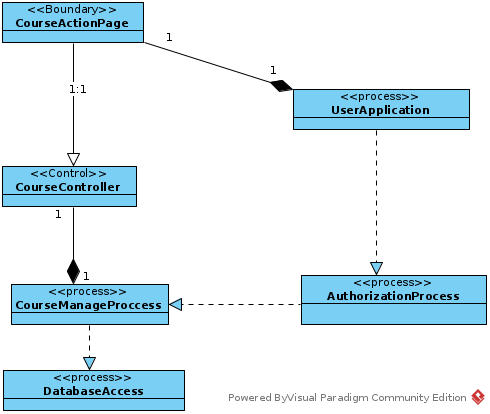
\includegraphics[width=\linewidth]{./images/pv_course_manage.png}
\end{figure}

\subsubsection{Mô tả các phần tử tiến trình}
\begin{itemize}
	\item Tiến trình CourseListApplication: Cung cấp giao diện, chức năng liên quan đến quản lý danh sách khóa học. Có một thể hiện của tiến trình này tương ứng với mỗi khách đăng nhập hệ thống.
	\item Tiến trình AuthorizationProcess: Quản lý quá trình thực hiện kiểm tra quyền truy cập tài khoản người dùng.
	Có một thể hiện của tiến trình này tương ứng mỗi lần khách truy cập trên hệ thống.
\item Tiến trình CourseManageProcess: Quản lý quá trình xử lý các yêu cầu liên quan tới khóa học.
	Có một thể hiện cho mỗi yêu cầu người dùng lên hệ thống.
	\item Tiến trình DatabaseAccess: Quản lý, xử lý các yêu cầu và thao tác liên quan đến database của hệ thống. Có nhiều thể hiện của tiến trình tương ứng với các database của hệ thống kết nối đến.
\end{itemize}

\end{document}